La mamá de Dmitri le hace una tienda para que vaya a acampar con sus amigos,
como la que se muestra en la figura \ref{fig:prob_verb_superficie_03}.
\textbf{¿Cuánto material necesitará la mamá de Dmitri para hacer la tienda, incluyendo el piso?}
\textit{Escribe una respuestan exacta (no redondees).}

\begin{minipage}{0.3\linewidth}
    \begin{figure}[H]
        \begin{center}
            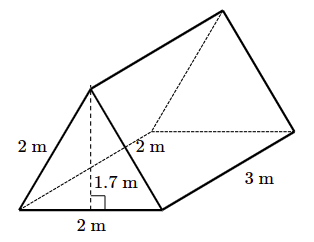
\includegraphics[width=1\textwidth]{../images/prob_verb_superficie_03}
        \end{center}
        \caption{}
        \label{fig:prob_verb_superficie_03}
    \end{figure}
\end{minipage}
\begin{minipage}{0.7\linewidth}
    \begin{solutionbox}{6cm}
    \end{solutionbox}
\end{minipage}